\documentclass[../../main.tex]{subfiles}

 \lhead{User Testing}
 
\begin{document}

\section{User Testing}
	Once the implementation of the system to allow the user to move themselves around a virtual space had been completed, the plausibility of the methods used were tested. The following sections present the aims of the user tests in full and the procedure required to fulfil the set objectives.

	\subsection{User Testing Aims}
		There were a total of 3 user tests, with the third being split into two parts with an identical procedure. The aims of each test were as follows:

		\textbf{Test \#1:} Investigate the effect of using the synthetic \ac{RIR}'s as opposed to the previously used real \ac{RIR}'s used.

		\textbf{Test \#2:} Investigate how far the user has to be moved before they notice that have been moved using synthetic \ac{RIR}'s

		\textbf{Test \#3.1:} Investigate which \ac{RIR} grid provides the user with the best sense of mobility

		\textbf{Test \#3.2:}  Investigate whether the users opinion changes when using a position feedback system


	\subsection{Testing Procedure}
		Before the tests were conducted, each participant was presented with a `Test Participant Form', informing them of the aims of the tests and the procedures that were to follow. As they were going to be stood inside the speaker array, the answers provided by each participant were taken down on their behalf. At the end of the experiment the answers were checked and signed by the participant assuring that their answers had been taken down accurately. The form provided to the participants can be found in~\nameref{appendixD}.

		\subsubsection{Test \#1}

			To test the effect of using sysnthetic \ac{RIR}'s as opposed to real \ac{RIR}'s the use was asked to perform the same takst twice. the taks 

			To investigate the difference in the perception of distance moved when using either synthetic or real \ac{RIR}'s, the following procedure was carried out:

			Figure~\ref{test1Positions} shows an illustration of the virtual space indicating where the four \ac{RIR} locations used for the test are. The black numbers indicate the coordinates of the \ac{RIR}'s  relative to the top left corner of the room (note that the x and y axis are opposite to convention due to the way the building was modelled in Google SketchUp), and the red numbers are used to indicate which location the user was moved to during each test, shown in table~\ref{test1Procedure}.


			The user was placed at position (1), in the centre of the virtual space and asked to say the word `Bob'. The were then moved to a new position and asked to repeat themselves


			%-------------Latency Diagram-------------%
			\begin{figure}[H]
				\centerline{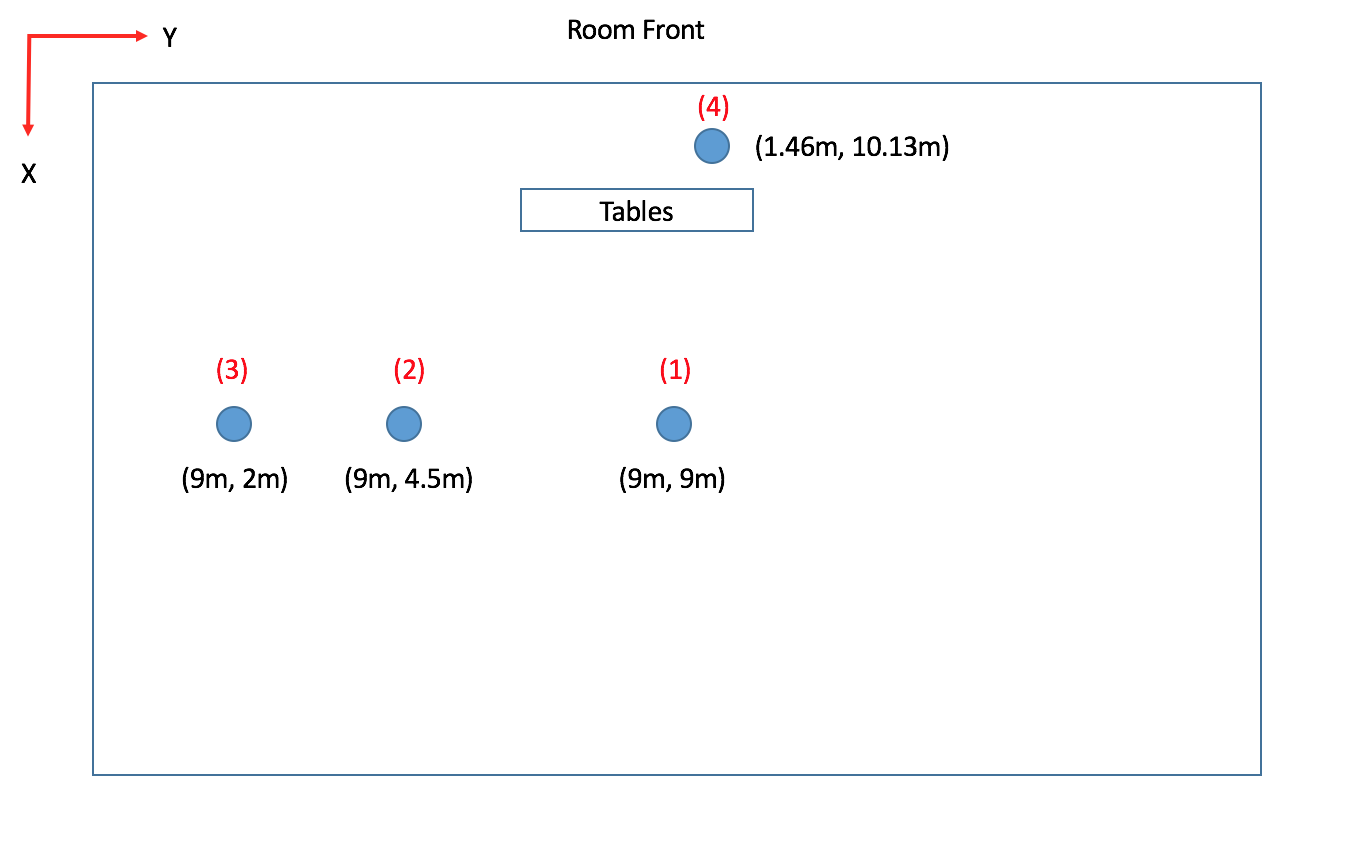
\includegraphics[scale = 0.5]{Sections/userTesting/images/test1/roomPositions3.png}}
				\caption{Illustration of \ac{RIR} locations used for user test \#1.}
				\label{test1Positions}
			\end{figure}



			% \begin{center}
			%     \begin{tabular}{|c|c|c|c|c|} \hline
			%         \multirow{2}{*}{Trail} & \multicolumn{2}{c|}{A} & \multicolumn{2}{c|}{B}\\ \cline{2-5}
			%             & Start & End & A & B \\ \hline
			          
			%           1 & (9,9)R & (9,4.5)R & (9,9)S & (9,4.5)S \\
			%           2 & (9,9)R & (9,2)R & (9,9)S & (9,2)S \\
			%           3 & (9,9)R & (1.17,10)R &  (9,9)S & (1.17,10)\\ \hline
			%           4 & (9,9)R & (9,2)R & (9,9)S & (1.17, 10)S  \\ 
			%           5 & (1.17, 10)R & (9,9)S & (9,9)S & (9,2)S \\ \hline
			%     \end{tabular}
			% \end{center}

			\begin{table}[H]
				\begin{center}
				    \begin{tabular}{|c|cc|cc|} \hline
				        \multirow{2}{*}{Trail} & \multicolumn{2}{c|}{Real RIR} & \multicolumn{2}{c|}{Odeon RIR}\\ \cline{2-5}
				            & Start & End & Start & End \\ \hline
				          1 & (1) & (2) & (1) & (2) \\
				          2 & (1) & (3) & (1) & (3)\\
				          3 & (1) & (4) & (1) & (4)\\ \hline
				          4 & (1) & (3) & (1) & (4)  \\ 
				          5 & (4) & (1) & (1) & (3) \\ \hline
				    \end{tabular}
				    \caption{Showing}
				    \label{test1Procedure}
				\end{center}
			\end{table}


		\subsubsection{Test \#2}

		\subsubsection{Test \#3}


	\subsection{Results}

		\subsubsection{Test \#1 Results}
		\subsubsection{Test \#1 Discussion}

		\subsubsection{Test \#2 Results}
		\subsubsection{Test \#2 Discussion}

		\subsubsection{Test \#3 Results}
		\subsubsection{Test \#3 Discussion}

	\subsection{Discussion}
	%Less RIRs, move faster, not good

\end{document}